\documentclass{article}
\usepackage{graphicx}
\usepackage[margin=2cm]{geometry}

\usepackage{titlesec}
\newcommand{\sectionbreak}{\clearpage}

\title{Dynamic Voxel Scenes using a Sparse Voxel Directed Acyclic Graph}
\author{Nicolas Fedor, 6683787}
\date{May 2025}

\begin{document}
\maketitle

\section{Introduction}
Voxel rendering has become an essential technique in computer graphics, enabling the representation and visualization of 3D environments through volumetric data. Unlike traditional polygon-based methods that rely on triangles and surface meshes, voxel rendering represents scenes as a grid of volumetric elements (voxels), which allows for detailed depictions of complex structures such as terrains, clouds, or medical imaging data. This approach offers several advantages, particularly in handling volumetric and procedural data, but also poses significant challenges, including high memory consumption and computational demands.

Several data compression techniques have been developed to address these challenges, such as Sparse Voxel Octrees (SVOs) and Sparse Voxel Directed Acyclic Graphs (SVDAGs). These methods aim to reduce memory usage by representing voxel data in a hierarchical, sparse format, allowing for efficient storage and rendering of large voxel grids. However, dynamic scenes present additional challenges, as updating the voxel data structure in real-time can be computationally expensive.

This project will explore the usage of SVDAGs for rendering large worlds and the challenges of dynamic voxel data. By optimising the construction of the SVDAG and separating static and dynamic voxel data, this work aims to achieve real-time rendering of dynamic voxel worlds with minimal memory footprint.

\subsection{Aims and Objectives}
The aim of this project is to develop a dynamic voxel rendering system using an SVDAG data structure. The objectives of this project are as follows:

\begin{itemize}
    \item Design and implement an SVDAG data structure for representing voxel data.
    \item Optimize SVDAG construction and traversal for real-time rendering.
    \item Allow for dynamic updates to an SVDAG to support interactive voxel worlds.
    \item Evaluate the performance of the dynamic voxel rendering system in terms of rendering speed and memory usage.
\end{itemize}

\section{Literature Review}
This chapter will provide an overview of the existing techniques for rendering voxel data, including traditional mesh-based methods and recent advances using ray tracing and sparse voxel representations.

\subsection{Mesh-based Rendering}
Mesh-based rendering is the most common technique for representing 3D objects in computer graphics. It involves defining the surface of an object using a collection of polygons, typically triangles, which are then rendered using the GPU's rasterization pipeline. This is a well-established approach, that is the default method for rendering 3D graphics in most applications.

Volumetric voxel data can be converted to a mesh representation using techniques such as Marching Cubes~\cite{Amran_1998}, which extract the surface of the volume by sampling the voxel data; or another simpler, popular, approach is to use greedy meshing~\cite{mikolalysenko_2012}, which relies on creating a mesh by merging adjacent voxels with the same material into a single quad face in the mesh. These approaches allow for storing voxel data uncompressed and so dynamic updates to voxel data are quick. However, the generation of the mesh becomes a bottleneck as the resolution of the voxel data increases. Additionally, meshes require a large amount of memory to store the vertex and index data, which can be a limiting factor for large voxel worlds; as more vertex attributes are required the memory usage increases, limiting the size of the voxel world that can be rendered.

\subsection{Ray Marching}
Ray marching, a specialized form of ray tracing, is another technique for rendering voxel data. It involves casting a ray through a 3D grid of voxels and sampling the voxel data along the ray to determine the color and opacity of the volume at each point. Ray marching can be implemented on the GPU using compute shaders, avoiding the creation of a mesh, instead the GPU can operate directly on the voxel data, which can be stored in a compressed format.

\subsubsection{Digital Differential Analysis (DDA)}
A common technique for ray marching is Digital Differential Analysis (DDA), which involves stepping through the voxel grid along the ray using fixed-size increments or steps calculated based on the ray direction. At each step, the voxel data is sampled to determine the color and opacity of the volume, which is accumulated along the ray to produce the final image. DDA is a simple and efficient method for ray marching~\cite{Amanatides_Woo_1987}, but intersection testing a ray is an expensive operation and so limiting the number of intersection tests a ray tracer must perform is important for real-time rendering.

\subsection{Data Compression}
Compression a voxel grid is essential for rendering large voxel worlds efficiently using ray marching as the number of intersection tests has a large impact on ray tracing performance, in ray tracing Binary Space Partitioning is a way of improving ray tracing performance~\cite{Ize_2009}. Sparse Voxel Octrees (SVOs) and Sparse Voxel Directed Acyclic Graphs (SVDAGs) are two common techniques for compressing voxel data, which store the voxel grid in a hierarchical, sparse format that can help reduce the number of intersection tests.

SVOs are a hierarchical data structure that represents a voxel grid as a tree of nodes, where each node contains either a single voxel or a pointer to a child node; the aim here is to reduce the memory usage by storing only the voxels that are necessary to represent the volume i.e. by collapsing "chunks" of similar voxels into a single node. An example of an SVO is shown in Figure~\ref{fig:svo}.

\begin{figure}[thp]
    \begin{center}
        \scalebox{0.5}{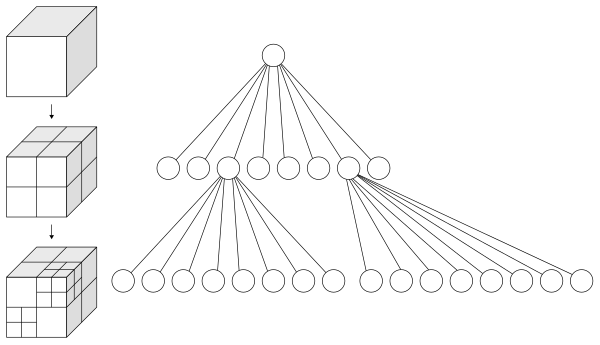
\includegraphics[width=0.8\textwidth]{figures/octree.png}}
    \end{center}
    \caption{Illustration of a Sparse Voxel Octree (SVO) representation of a voxel grid.}
    \label{fig:svo}
\end{figure}

SVDAGs build upon a similar idea to SVOs, but instead of using a tree structure, they use a directed acyclic graph (DAG) to represent the voxel data. This allows for further reducing duplication of data by instead storing pointers to shared subgraphs of the DAG.

SVOs and SVDAGs~\cite{Kampe_Sintorn_Assarsson} are both popular approaches for rendering large amounts of voxels with a minimal footprint, while also reducing the amount of potential intersection tests a DDA ray tracer must perform. However, updating the voxel data in real-time can be challenging, as modifying the structure of the SVO or SVDAG can be computationally expensive. Recent papers have proposed techniques for dynamic updates to SVDAGs~\cite{Careil_Billeter_Eisemann_2020} by separating static and dynamic voxel data, allowing for efficient updates to the voxel grid while maintaining real-time rendering performance. The additional compression of an SVDAG compared to an SVO can be seen in Figure~\ref{fig:svdag}.

\begin{figure}[thp]
    \begin{center}
        \scalebox{0.5}{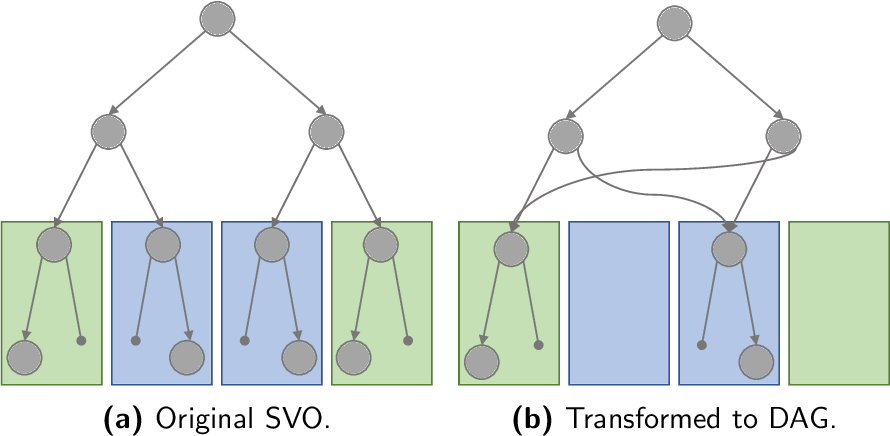
\includegraphics[width=0.8\textwidth]{figures/svdag.png}}
    \end{center}
    \caption{Illustration of the compression on an SVDAG compared to an SVO. The green and blue nodes represent identical subtrees in the SVO. For simplicity, the octree is shown as a binary tree.}
    \label{fig:svdag}
\end{figure}

\section{Technical Overview}
This chapter will provide a technical overview of the proposed dynamic voxel rendering system using an SVDAG data structure, based on the literature review and the project objectives.

\subsection{Sparse Voxel Directed Acyclic Graphs}

\subsection{Dynamic Voxel Data}

\section{Workplan}
The following work plan is what I will be using for the project is shown in Figure.

\bibliographystyle{IEEEtran}
\bibliography{references}

\end{document}
